This section discusses the implementation of the algorithm, the problems encountered and a comparison with the latest Cuckoo version.

\subsection{Implementing the algorithm}

The actual code can be found on GitHub at \url{https://github.com/MartijnB/cuckoo/tree/multi-url}.

%\subsubsection{Step 1: Visit}
\begin{enumerate}
\item \textbf{Visit} To support the parallel visiting of URLs in one virtual machine, Cuckoo had to be extended. Support for this was added pretty quickly using tabs, but this left us with a problem to detect when a new URL was feeded to a tab\todo{See problems below}. To solve this problem, every URL in this PoC is now opened in its own window.

%\subsubsection{Step 2: Process}

\item \textbf{Process} In this step, the API calls were bundled into ten different events before being added to the graph. If no relation was found between an event and a previous event, an edge was created from the event to the event which represents the browser context. The HTTP `Referer' header was used to find relations between HTTP events, essentially creating a referer tree.\cite{http://pdf.aminer.org/000/654/566/analysis_of_user_web_traffic_with_a_focus_on_search.pdf} \todo{Define all relations here?}

%\subsubsection{Step 3: Analyze}

\item \textbf{Analyze} To implement the analysis phase of the algorithm, a simple analyzer was written that detects process spawns below browsing contexts. Listing \todo{reffie} shows pseudo code of the analyzer.

\begin{lstlisting}
function deep_process_spawn_analyzer(graph)
    foreach vertex in graph
        if vertex.type == "process_spawned"
            if check_depth_in_graph(vertex, 0) > 1
                print "Malicious activity"
            endif
        endif
    endforeach
endfunction

function check_depth_in_graph(vertex, current_depth)
    parents = get_parents_of_vertex(vertex)
    # Actually we need only one parent
    if length_array(parents) > 0
        return check_depth_in_graph(parents[0], current_depth++)
    else
        # No more parents, we're at the root node
        return current_depth
    endif
endfunction
\end{lstlisting}

%\subsubsection{Step 4: Report}

\item \textbf{Report} Reporting is done on the commandline but generated graphs of anomalities are saved to the disk in the folder structure of Cuckoo.
\end{enumerate}

\subsubsection{Problems}
\label{99problems}
\epigraph{I've got 99 problems but Cuckoo ain't one.}{Adriaan}

During the development of the proof of concept, several problems were encountered. We discuss the most interesting ones here.

\textbf{Opening a new URL in the same browser context} was not detectable by the monitored API calls. Additionally processes were reused when a browsing context was closed and a new one was openened, this made it essentially the same as reusing the browsing context. Internet Explorer also behaves differently when interacting with the COM interface compared to real user interaction, leaving us without certain registry values that could be used to detect the opening of a new URL. Therefor we decided to use a new Internet Explorer process for each URL which gives us a process ID per browser context.

\subsection{Running the PoC}

Running the proof of concept is as simple as running Cuckoo and running our Python script. Listing \todo{reffie} shows how the PoC is run. As explained in section \todo{reffie} the URL list contains the Top 20 most visited websites and some malware websites. Figure \ref{graph} shows the full graph created in the process phase. Notice the red dots in the top left corner of the graph which indicate process spawns. The analyzer run in phase 3 succesfully found this anomality and reports it back to the user. A graph of the browsing context in which this anomality occured is also shown to the user, as can be seen in figure \ref{fig:subgraph}.

\begin{lstlisting}
$ python cuckoo.py &
$ python utils/mass-analyse.py url_list.txt
Warning: Task with ID 22 is not yet completed; Waiting...
INFO:root:Parse log....
Analyzer 'Subprocess_from_tab': The URL 'http://malware-site.com' 
spawns a process called 'errfix.exe'.
\end{lstlisting}

\begin{figure}[h]
    \centering
    \centerline{\includegraphics[width=20cm]{Images/graph4.jpg}}
    \caption{An example of the graph}
    \label{fig:graph}
\end{figure}

\newgeometry{left=3cm,top=0.1cm,bottom=0.1cm}
\begin{figure}[h]
    \centering
    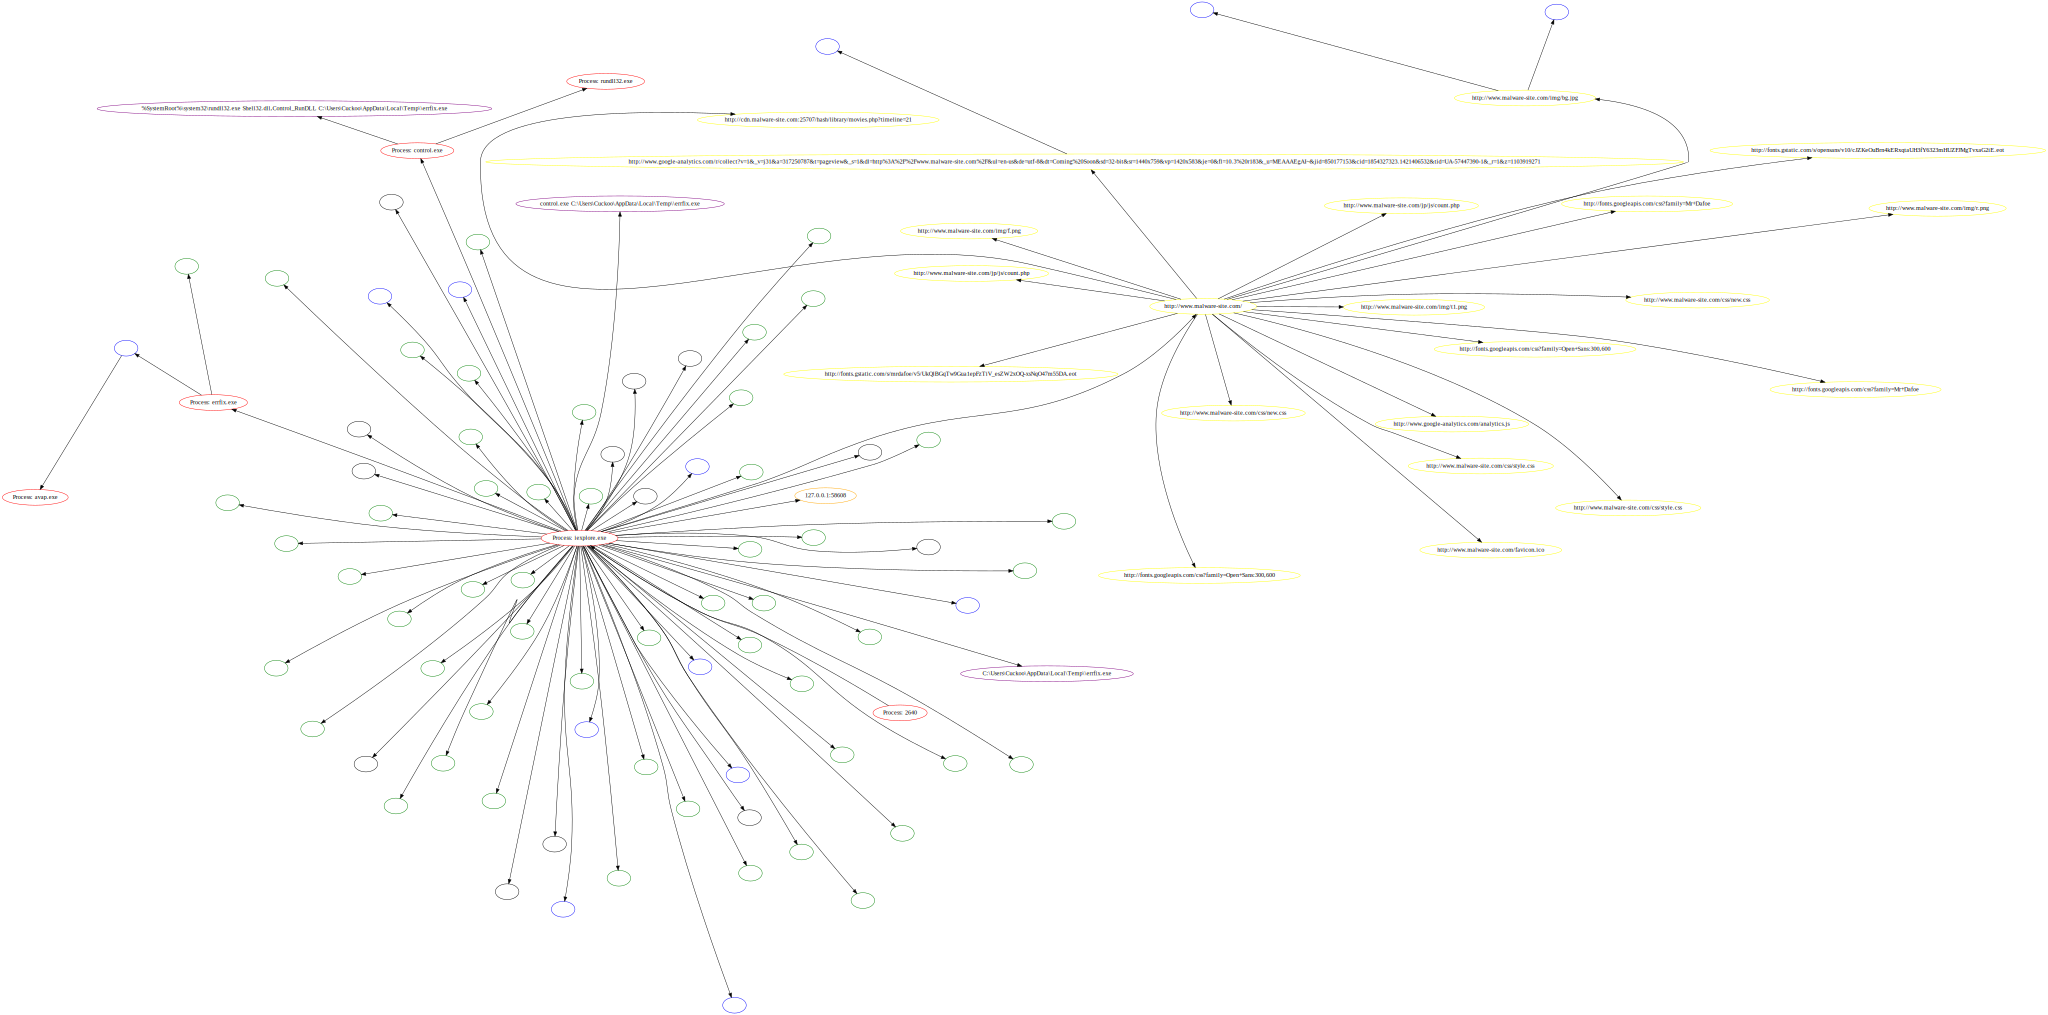
\includegraphics[width=25cm, angle=90]{Images/report_Subprocess_from_tab}
    \caption{An example of the subgraph of a single website that infected the virtual machine with malware. For clarity are only the labels showed of the nodes of visited URLs, involved processes and executed shell commands.}
    \label{fig:subgraph}
\end{figure}

\restoregeometry
\subsection{Comparison with Cuckoo 1.2}

Doe een keer voor vijf URLs, voor 10 URLs, voor 15 URLs, voor 20 URLs,...
Daar kan je wel een grafiekje van maken dan, ook perfect om te doen
als we in het lab zitten, aangezien we dan toch altijd slacken

\todo{Speedboost tussen Cuckoo 1.2-dev en onze wijzigingen in grafiekje zetten}
